\chapter{GoF}
\section{Introducción}
\newpage

\section{Patrones Creacionales}
\newpage


\subsection{Fabrica abtsracta}
Descripción
%%modelo
\begin{figure}[th!]
	\centering
	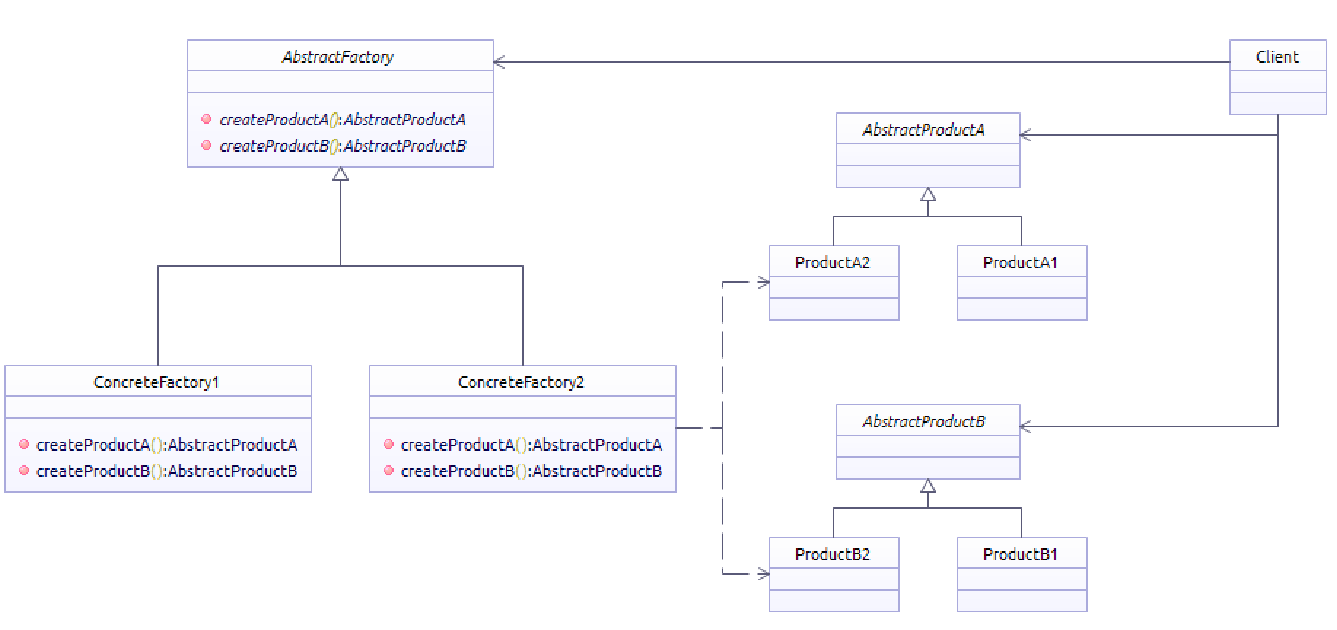
\includegraphics[width=0.7\linewidth]{arquitectura/diseno/imgs/m_fabrica}
	\caption{Fabrica Abstracta}
\end{figure}

\newpage

\subsubsection{Caso}

\begin{figure}[th!]
	\centering
	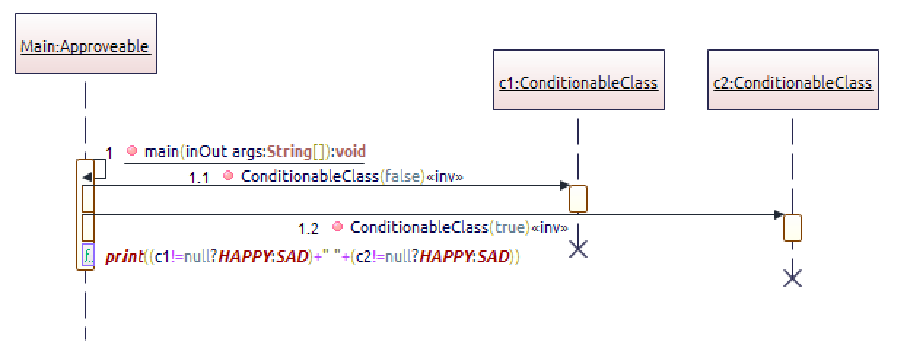
\includegraphics[width=0.7\linewidth]{arquitectura/diseno/imgs/s_fabrica}
	\caption{Fabrica Abstracta}
\end{figure}

\newpage


\section{Patrones Estructurales}
\newpage


\section{Patrones de Comportamiento}
\newpage



